\chapter{Description of AsthmAPP}
\label{chp:description}

This chapter will give a description of AsthmAPP, through textual description and screen shots. Please note that the main language of the application is Norwegian, and we have translated parts of it where it seems appropriate. 

\section{Basic System Architecture}
\label{sec:architecture}
Figure \ref{fig:basic-architecture} shows an overview of the architecture we intend to use for our solution. We will build upon the architecture used by Aaberg et. al. \cite{CustomerDriven}.

We have access to a MySQL-server hosted at NTNU, which we will access by a PHP-server hosted at NTNU. The main reason we have to access the database through a server layer, is that it is quite cumbersome to connect to the database if a device is not connected at NTNU's network. In addition, by having a webservice do some of the work for us, it becomes easier to parse results from the database through JSON.   


The downside by having this approach is that scalability suffers from this architectural choice. However, we consider these problems as outside the scope of our thesis, and will continue using this approach.

\begin{figure}
		\centering
			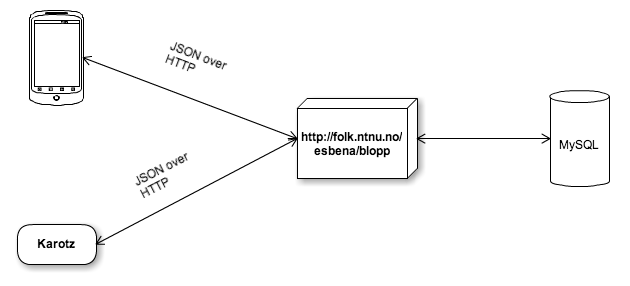
\includegraphics[width=0.50\paperwidth]{Pictures/basic-architecture.png}
		\caption{Basic architecture of our system}
		\label{fig:basic-architecture}
\end{figure}

\section{Child partition}
\label{sec:description-child-partition}
The child partition of our application consists mainly out of four parts. When Aaberg et. al. created the original application, they wanted a conceptual look and feel throughout the applications. They used images of Karotz in the application in order to introduce a sense of completeness, i.e. the Karotz bound CAPP, GAPP and KAPP together. [TODO: Vi burde bytte ut Karotz-bilder med eget produkt imo]. 

\subsection{Treatment}
\label{sec:sec:description-treatment}
Figure \ref{fig:capp_start_treatment} shows a screenshot for the application when the child starts their treatment. Starting this sequence can come from one out of two events: (i) \emph{The child reacts to an alarm set in the parent partition}, and (ii) \emph{The child needs to take their medicine by need}. If (ii) is the case, the child is instructed to pick the medicine from a list shown by the application. If (i) is the case, the medicine is chosen beforehand. When a child has started their treatment, they are taken through an animated sequence, which reacts when a child interacts with the device. In addition, they are being told what to do through the comforting voice of Yngve Svalestuen.  


\subsection{Showing rewards}
\label{sec:description-show-rewards}
Figure \ref{fig:capp_stars} shows a screenshot for the application when the child wants to review how many stars he/she has received, based on the amount of medicine they have taken. We have made two design decisions for our reward system. First, we never want stars to be removed. We don\'t want children to feel that credits are being removed from them. Second, we can\'t assume children are able to read, and thus we have made it countable, and hopefully they can comprehend how many stars they've actually got. In addition, we provide some help to those who are able to read numbers, by showing the amount of stars a child has on the top. The downside here comes when a child has been given a huge number of treatment, such as 200 treatments or more. This will obscure the view.     

\subsection{Shop}
\label{sec:description-shop}
In the shop, children are allowed to buy rewards from parents [Insert Reference]. Figure \ref{fig:capp_store} shows a inside-view of our shop. Children can buy an activity by pressing the selected activity. Due to time constraints, we have not been able to implement voice over, so the children will have to find a parent who can read it if they are not able to [TODO: 1: Bryter med linjen over. 2: Implementasjon av voice over med norsk som språk er vanskelig]. 



\subsection{Treatment instructions}
\label{sec:description-instructions}
The treatment instructions is a book-styled instruction set which shows generically how to take a medicine. 
The following steps are included in instructions: 
\begin{enumerate}
  \item Shake the inhaler such that the particles loosen up. 
  \item Take the cap of the inhaler
  \item Attach the inhaler to the inhaling chamber [TODO: Korrekt bruk av chamber?]
  \item Put the inhaler onto the face of the child
  \item Press the inhaler until you hear a sound
  \item Let the child breathe calmly 10 times in and out
  \item Let the child wash his/her mouth
\end{enumerate} 



\begin{figure}
	\begin{minipage}[b]{0.4\linewidth}
		\centering
			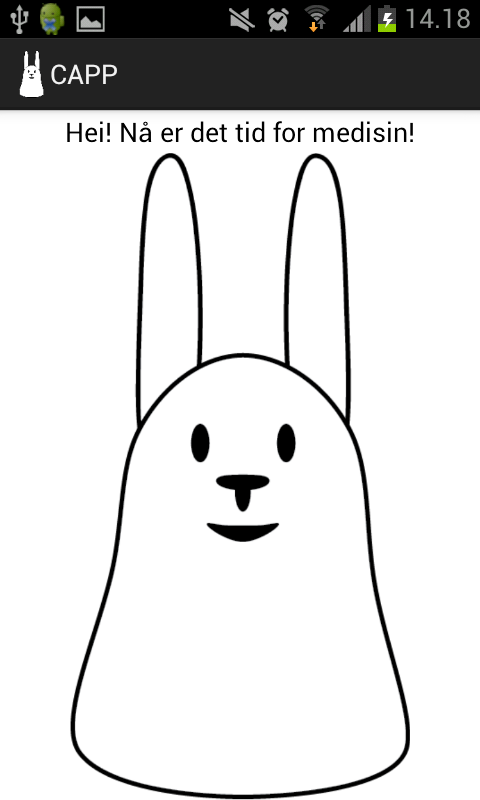
\includegraphics[width=0.20\paperwidth]{Pictures/app-screenshots/capp_start_treatment.png}
		\caption{Starting a treatment}
		\label{fig:capp_start_treatment}
	\end{minipage}
	\hspace{3cm}
	\begin{minipage}[b]{0.4\linewidth}
		\centering
			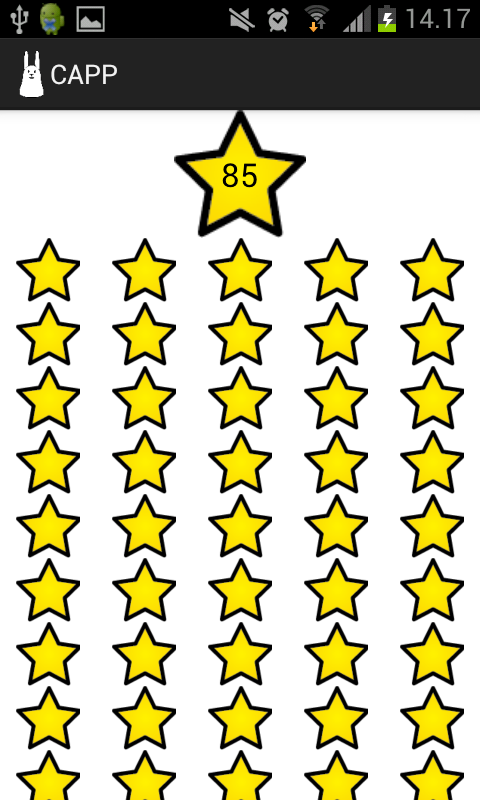
\includegraphics[width=0.20\paperwidth]{Pictures/app-screenshots/capp_stars.png}
		\caption{SHOULD BE A SHOP}
		\label{fig:capp_store}
	\end{minipage} 
\end{figure}
% 
% \begin{figure}
% 	\begin{minipage}[b]{0.3\linewidth}
% 		\centering
% 		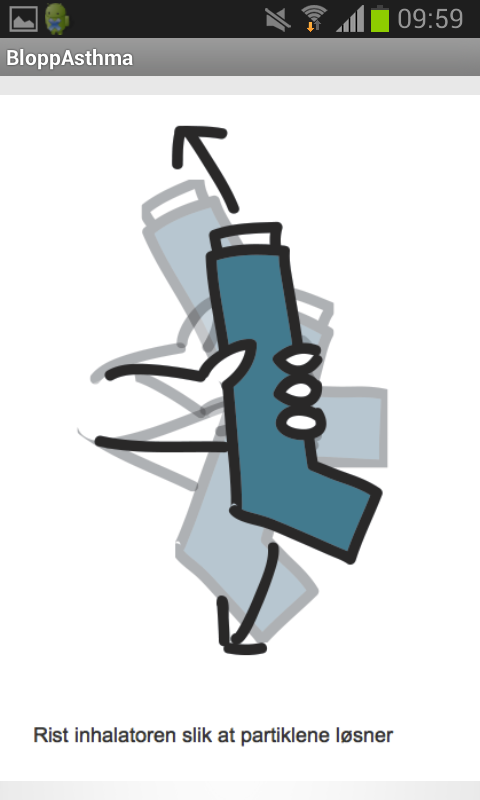
\includegraphics[width=0.20\paperwidth]{Pictures/app-screenshots/instructions-1.png}
% 		\caption{Instructions 1}
% 		\label{fig:instructions-1}
% 	\end{minipage}
% 	\begin{minipage}[b]{0.3\linewidth}
% 		\centering
% 		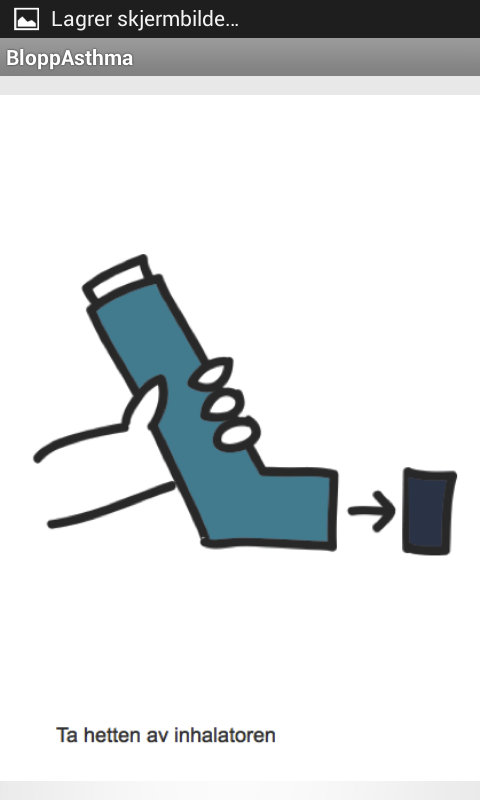
\includegraphics[width=0.20\paperwidth]{Pictures/app-screenshots/instructions-2.png}
% 		\caption{Instructions 2}
% 		\label{fig:instructions-2}
% 	\end{minipage}
% 	\begin{minipage}[b]{0.3\linewidth}
% 		\centering
% 		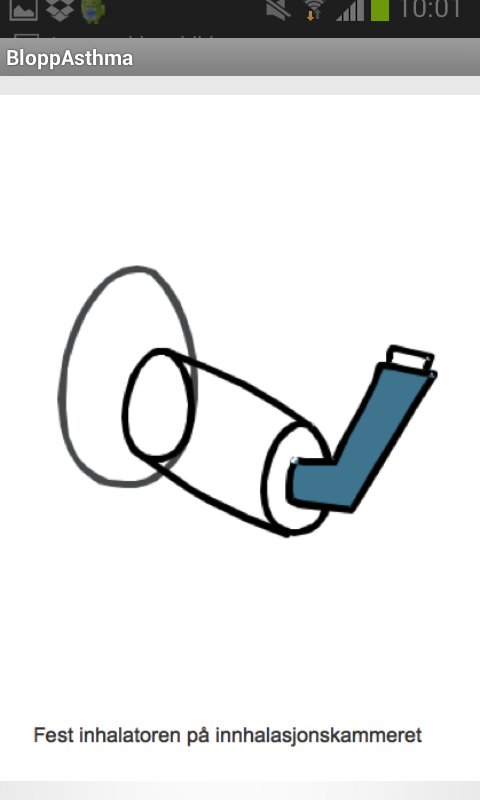
\includegraphics[width=0.20\paperwidth]{Pictures/app-screenshots/instructions-3.png}
% 		\caption{Instructions 3}
% 		\label{fig:instructions-3}
% 	\end{minipage}
% 	
% 	\begin{minipage}[b]{0.3\linewidth}
% 		\centering
% 		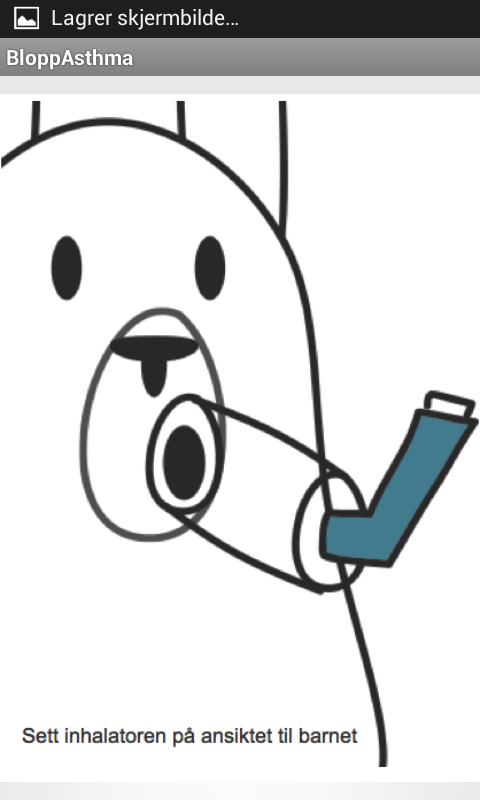
\includegraphics[width=0.20\paperwidth]{Pictures/app-screenshots/instructions-4.png}
% 		\caption{Instructions 4}
% 		\label{fig:instructions-4}
% 	\end{minipage}
% 	\begin{minipage}[b]{0.3\linewidth}
% 		\centering
% 		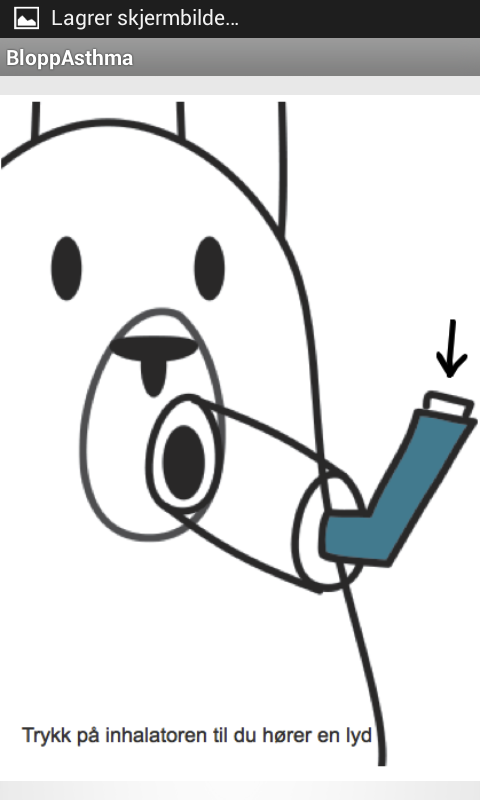
\includegraphics[width=0.20\paperwidth]{Pictures/app-screenshots/instructions-5.png}
% 		\caption{Instructions 5}
% 		\label{fig:instructions-5}
% 	\end{minipage}
% 	\begin{minipage}[b]{0.3\linewidth}
% 		\centering
% 		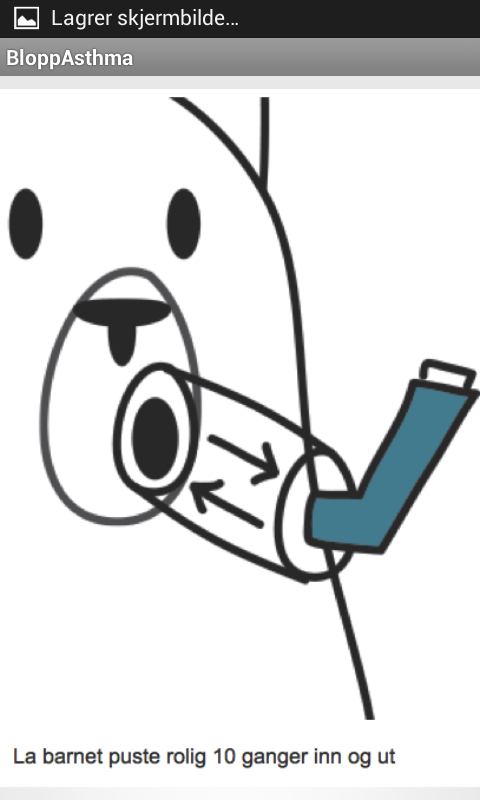
\includegraphics[width=0.20\paperwidth]{Pictures/app-screenshots/instructions-6.png}
% 		\caption{Instructions 6}
% 		\label{fig:instructions-6}
% 	\end{minipage}
% 	
% 	\begin{minipage}[b]{0.3\linewidth}
% 		\centering
% 		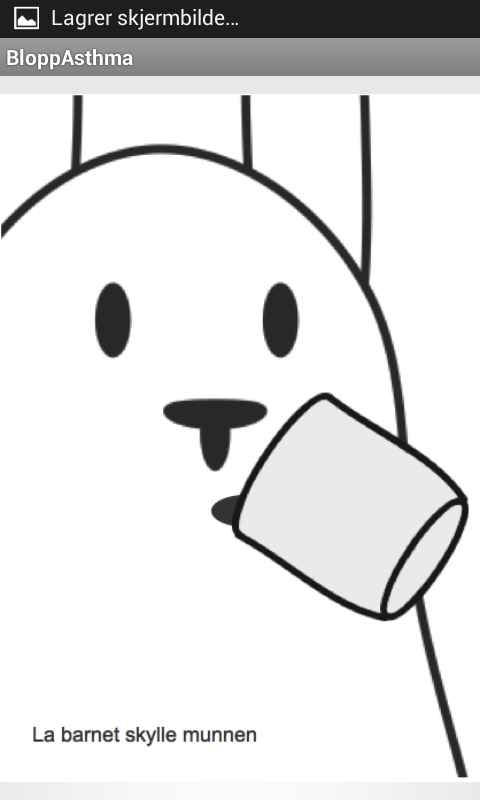
\includegraphics[width=0.20\paperwidth]{Pictures/app-screenshots/instructions-7.png}
% 		\caption{Instructions 7}
% 		\label{fig:instructions-7}
% 	\end{minipage}
% \end{figure}





\section{parent partition}
This section will take you through the parent partition of AsthmAPP.

\subsection{Menu}
\label{sec:description-menu}
Figure \ref{fig:gapp-main-menu} shows the main menu of the parent partition. It has six options (norwegian translation in paranthesis):
\begin{enumerate}
  \item Medicine Plan (\emph{Medisinplan})
  \item Register Medicine Afterwards (\emph{Etterregistrer medisin})
  \item Medicine Log (\emph{Medisinlogg})
  \item Medicine Information (\emph{Legemiddelinformasjon})
  \item Manual (\emph{Manual})
  \item Rewards (\emph{Premier})
\end{enumerate} 


\subsection{Medicine plan}
\label{sec:description-medicine-plan}
Creating a medicine plan for asthma treatment is highly connected to the Traffic Light System [INSERT REFERENCE].
Users can have three different plans, depending on which health state they are currently in. As we are targeting children, we can not assume that they are aware of which category they are currently in, and as a result, we let their parents control it. Figure \ref{fig:gapp-view-plans} and [INSERT REFERENCE TO EDIT PLAN] shows the view in which one may the change medicine plan their child are currently on, in addition to setting alarms where appropriate. For instance, one might set an alarm at 07:00, which makes the user aware before it is time to leave for school. Changing medicine plan is done by selecting the checkbox at the left side of the panel.  

\subsection{Register medicine}
\label{sec:description-register-medicine}
What happens if a child need their medicine, but the application or our TUI is not nearby? They would probably be mad because they did not get their star, and did not make any progress as far as the rewards go. Fortunately, it is possible to register a medicine that has been taken afterwards, which entitle the child the amount of stars they should have gotten. \emph{Register Medicine Afterwards} allows parents to register the medicine, at any given day prior to current time (See Figure \ref{fig:gapp-register-treatment}).  


\subsection{Medicine log}
\label{sec:description-medicine-log}
The \emph{Medicine log} can be used by parents to show how many times a child has taken their medicine. One of the main reasons that children does not take their medicine is lack of communication between parents. Having an option to show medicine log, give parents the ability to check and see whether they have taken the necessary amount at a given day.

Figure [INSERT REFERENCE] shows the calendar view of the application. The view is a bit complicated, and an explanation is in it's place. We'll start out by the cells in the calendar. They obviously show any given day of a month. In addition, there is a top bar in the view. The top bar indicates which health state (or health plan) the child was in at a given day. At the bottom of the screen, there are three panels. The left one shows which medicine that has been taken at a selected day. The middle one shows the air quality in Trondheim. The right shows the pollen distribution of the 6 most common pollen types. The idea behind this is that asthma symptoms can often be the same as allergy symptoms, and if parents are able to recongize a pattern between health state and pollen distribution, they might want to take their child to a hospital.   
 
\subsection{Medicine information}
\label{sec:description-medicine-information}
Figures \ref{fig:information-1} and \ref{fig:information-2} shows the application's medicine information functionality. The information part of the application is a part that is somewhat down-prioritized. At the time being, it contains a lightweight description of what it is, what it is used for, important information and how you apply it. 


\subsection{Manual}
\label{sec:description-manual}
The manual contains excactly the same information as shown in Section \ref{sec:description-instructions}. [TODO: Beskrive hvorfor dette er to steder i appen?]


\subsection{Reward}
\label{sec:description-manage-rewards}
Figure \ref{fig:reward-list} shows the list of possible rewards a child might receive. They are added by parents through \emph{Add reward}. The idea of having parents set their children's rewards is to specify rewards according to children's interest [TODO: Referanse til hvor vi har sagt dette før]. Figure \ref{fig:add-reward} shows how one may add an activity. Users inserts a description, then either take a photo or select one out of our standard images. It is possible to set a reward on ``Repeat'', which will make the reward repeating with twice the amount of stars [TODO: Omformuler].        
When the user press \emph{Save} (Lagre), the reward is added and children have the possibility to buy it. 
 
% 
% \begin{figure}
% 	\begin{minipage}[b]{0.3\linewidth}
% 		\centering
% 		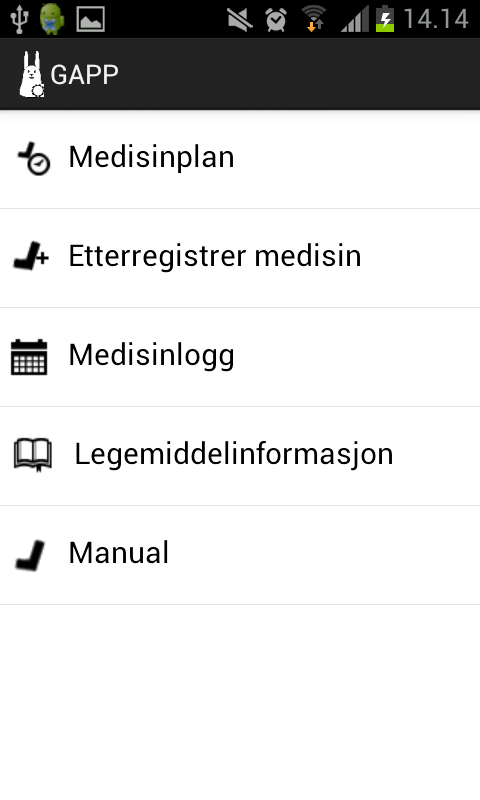
\includegraphics[width=0.20\paperwidth]{Pictures/app-screenshots/gapp_main_menu.png}
% 		\caption{Menu in parent partition}
% 		\label{fig:gapp-main-menu}
% 	\end{minipage}
% 	\begin{minipage}[b]{0.3\linewidth}
% 		\centering
% 		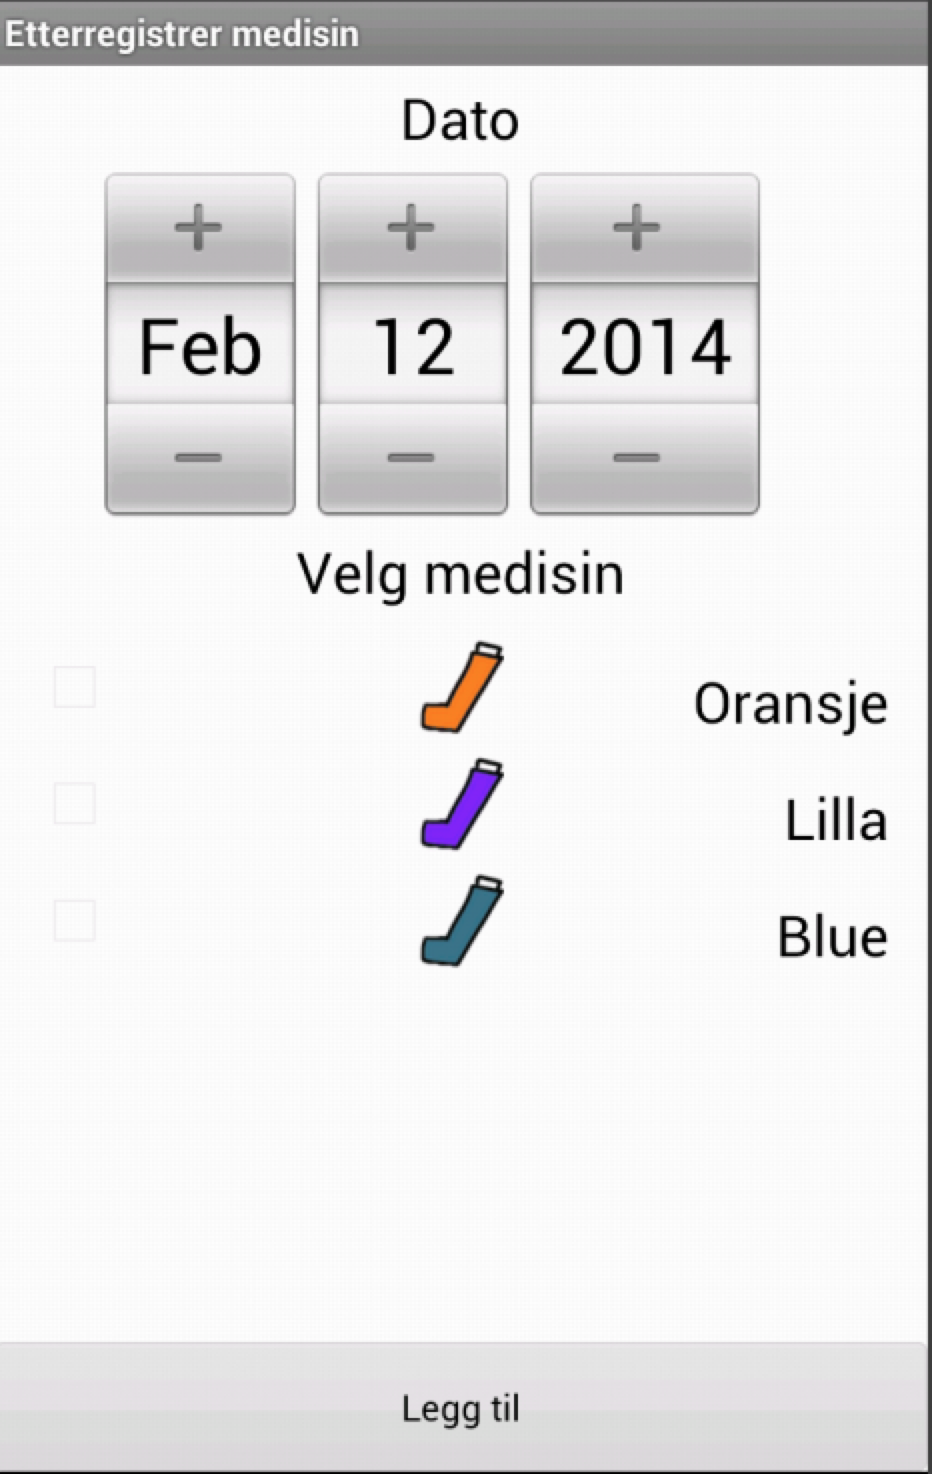
\includegraphics[width=0.20\paperwidth]{Pictures/app-screenshots/register_treatment.png}
% 		\caption{Register treatment}
% 		\label{fig:gapp-register-treatment}
% 	\end{minipage}
% 	\begin{minipage}[b]{0.3\linewidth}
% 		\centering
% 		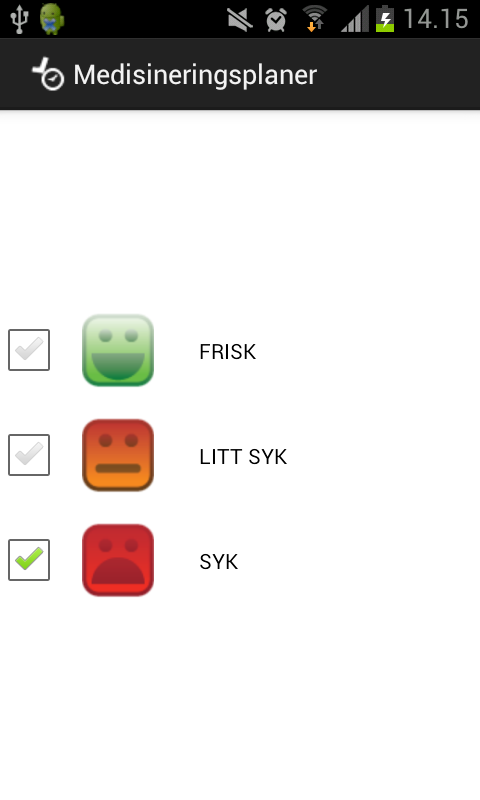
\includegraphics[width=0.20\paperwidth]{Pictures/app-screenshots/gapp_view_plans.png}
% 		\caption{View plans}
% 		\label{fig:gapp-view-plans}
% 	\end{minipage}
% 	\begin{minipage}[b]{0.3\linewidth}
% 		\centering
% 		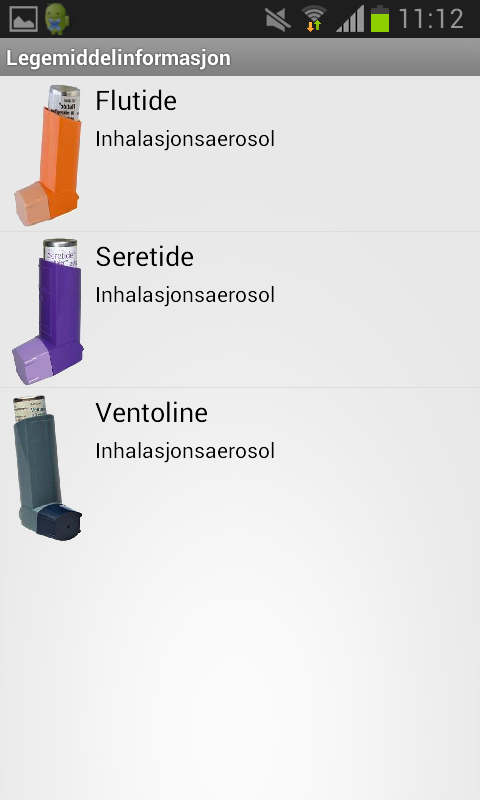
\includegraphics[width=0.20\paperwidth]{Pictures/app-screenshots/information-1.png}
% 		\caption{Information 1}
% 		\label{fig:information-1}
% 	\end{minipage}
% 	\begin{minipage}[b]{0.3\linewidth}
% 		\centering
% 		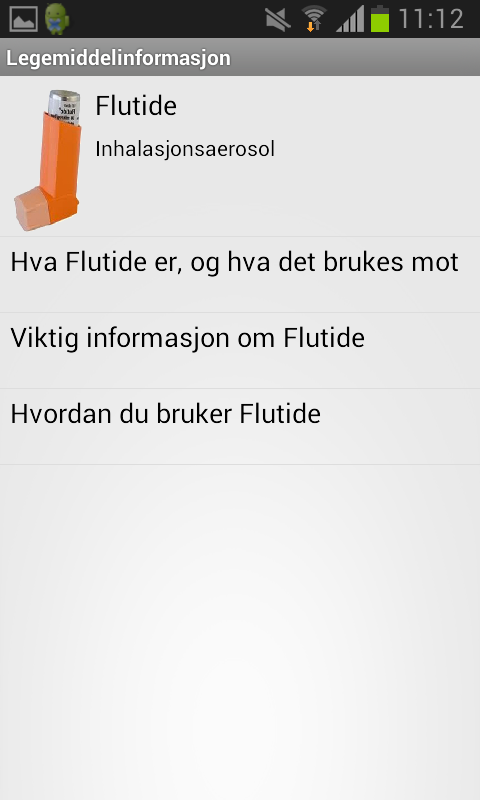
\includegraphics[width=0.20\paperwidth]{Pictures/app-screenshots/information-2.png}
% 		\caption{Information 2}
% 		\label{fig:information-2}
% 	\end{minipage}
% 	\begin{minipage}[b]{0.3\linewidth}
% 		\centering
% 		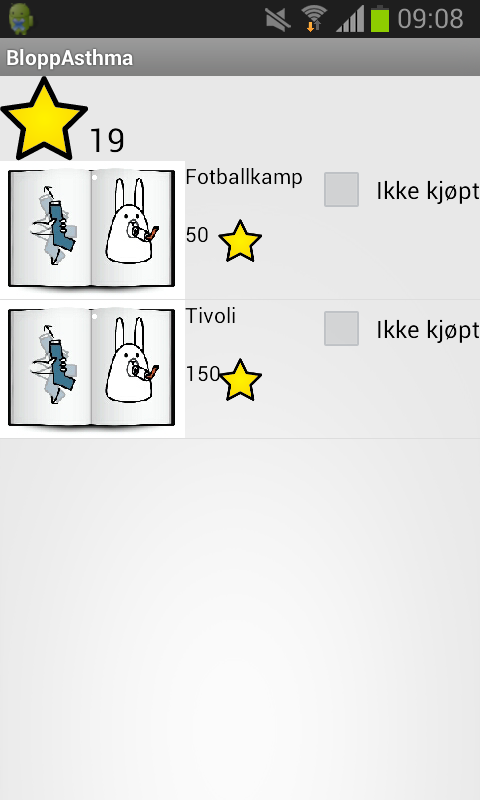
\includegraphics[width=0.20\paperwidth]{Pictures/app-screenshots/reward-list.png}
% 		\caption{Reward list}
% 		\label{fig:reward-list}
% 	\end{minipage}
% 	\begin{minipage}[b]{0.3\linewidth}
% 		\centering
% 		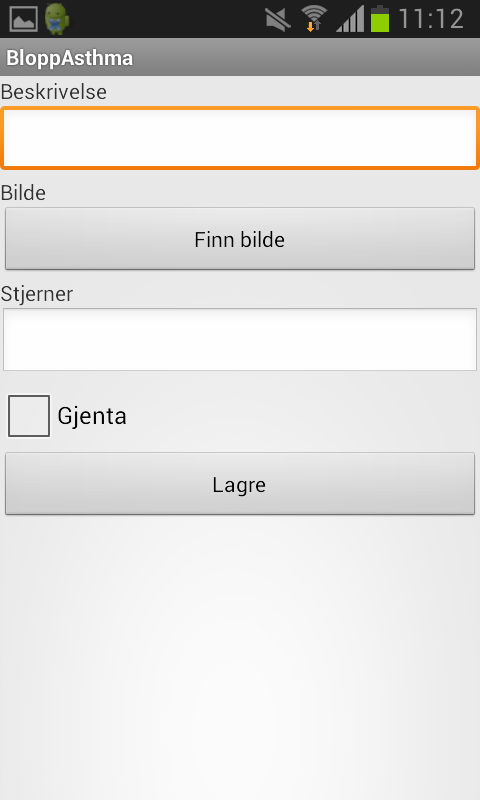
\includegraphics[width=0.20\paperwidth]{Pictures/app-screenshots/add-reward.png}
% 		\caption{Add reward}
% 		\label{fig:add-reward}
% 	\end{minipage}
% \end{figure}
% Skjermbilder -> Forklaringer
% Dropper alt som har med Karotz å gjøre, med unntak av ``konsept''-følelsen
% 